% --------------------------------------------------------------
% This is all preamble stuff that you don't have to worry about.
% Head down to where it says "Start here"
% --------------------------------------------------------------

\documentclass[12pt]{article}

\usepackage[margin=1in]{geometry} 
\usepackage{amsmath,amsthm,amssymb}
\usepackage{graphicx}

\newcommand{\N}{\mathbb{N}}
\newcommand{\Z}{\mathbb{Z}}

\newenvironment{theorem}[2][Theorem]{\begin{trivlist}
		\item[\hskip \labelsep {\bfseries #1}\hskip \labelsep {\bfseries #2.}]}{\end{trivlist}}
\newenvironment{lemma}[2][Lemma]{\begin{trivlist}
		\item[\hskip \labelsep {\bfseries #1}\hskip \labelsep {\bfseries #2.}]}{\end{trivlist}}
\newenvironment{exercise}[2][Exercise]{\begin{trivlist}
		\item[\hskip \labelsep {\bfseries #1}\hskip \labelsep {\bfseries #2.}]}{\end{trivlist}}
\newenvironment{reflection}[2][Reflection]{\begin{trivlist}
		\item[\hskip \labelsep {\bfseries #1}\hskip \labelsep {\bfseries #2.}]}{\end{trivlist}}
\newenvironment{proposition}[2][Proposition]{\begin{trivlist}
		\item[\hskip \labelsep {\bfseries #1}\hskip \labelsep {\bfseries #2.}]}{\end{trivlist}}
\newenvironment{corollary}[2][Corollary]{\begin{trivlist}
		\item[\hskip \labelsep {\bfseries #1}\hskip \labelsep {\bfseries #2.}]}{\end{trivlist}}

\begin{document}
	
	% --------------------------------------------------------------
	%                         Start here
	% --------------------------------------------------------------
	
	%\renewcommand{\qedsymbol}{\filledbox}
	
	
	\title{Computational Topology \\ Homework 1}
	\author{%replace with your name
		Bernarda Petek} %if necessary, replace with your course title
	
	\date{November 13, 2022}
	\maketitle
	

	
	\section{Theoretical problems}
    \subsection{Exploring different metrics} 
    
    \textbf{(a)} I determined the distances between points $(1,2), (2,4)$ and $(2,-1)$ in all three metrics. \\
    
    \noindent First, I determined the distances in metric $\alpha$. No two given points were the same so I always used the second part of the $\alpha$ distance definition:
    
    $$\alpha((1,2), (2,4)) = \sqrt{1^2 + 2^2} + \sqrt{2^2 + 4^2} = \sqrt{5} + \sqrt{20} = \sqrt{5} + \sqrt{4\cdot5} = \sqrt{5} + 2\cdot\sqrt{5} = 3\cdot\sqrt{5}$$
    $$\alpha((1,2), (2,-1)) = \sqrt{1^2 + 2^2} + \sqrt{2^2 + (-1)^2} = \sqrt{5} + \sqrt{5} = 2\cdot \sqrt{5}$$
    $$\alpha((2,4),(2,-1)) = \sqrt{2^2 + 4^2} + \sqrt{2^2 + (-1)^2} = \sqrt{20} + \sqrt{5} = 2\cdot\sqrt{5} + \sqrt{5} = 3\cdot\sqrt{5}$$
    
    \noindent Next, I determined the distances in metric $\beta$. Pair of points $(1,2)$ and $(2,4)$ satisfied the first condition (i.e. $1\cdot4=2\cdot2$), but the other two pairs of points $(1,2), (2,-1)$ and $(2,4),(2,-1)$ did not. ($1\cdot(-1)\neq2\cdot2$ and $2\cdot(-1)\neq2\cdot4$, respectively):
    
    $$\beta((1,2), (2,4)) = \sqrt{(1-2)^2 + (2-4)^2} = \sqrt{(-1)^2 + (-2)^2} =
    \sqrt{1+4}=\sqrt{5}$$
    $$\beta((1,2), (2,-1)) = \sqrt{1^2 + 2^2} + \sqrt{2^2 + (-1)^2} = \sqrt{5} + \sqrt{5} = 2\cdot \sqrt{5}$$
    $$\beta((2,4),(2,-1)) = \sqrt{2^2 + 4^2} + \sqrt{2^2 + (-1)^2} = \sqrt{20} + \sqrt{5} = 2\cdot\sqrt{5} + \sqrt{5} = 3\cdot\sqrt{5}$$
    
    \noindent Lastly, I determined the distances in metric $\gamma$. The first pair of points $(1,2), (2,4)$ did not satisfy the first condition: $1\neq2$. The second pair of points $(1,2), (2,-1)$ also did not satisfy the first condition: $1\neq2$. However, the last pair of points $(2,4),(2,-1)$ did satisfy the first condition: $2=2$. 
    
    $$\gamma((1,2), (2,4)) = |2| + |2-1| + |4| = |2| + |1| + |4| = 7 $$
    $$\gamma((1,2), (2,-1)) = |2| + |2-1| + |-1| = |2| + |1| + |-1| = 2 + 1 + 1 = 4  $$
    $$\gamma((2,4),(2,-1)) = |-1-4| = |-5| = 5$$
    
    \textbf{(b)} I drew the open balls $B((0,0), 1)$, $B((0,1), 2)$ and $B((1,2), 1 + \sqrt{5})$ in $\alpha$ metric. The centre of the ball is always contained in it because the $\alpha$ distance from and to itself is always $0$ (first condition) and $0$ is always smaller than the radius $r>0$ of the open ball. The drawings can be seen on Figures $1, 2$ and $3$. The calculations I made were: 
    
    \begin{figure}
    	\centering
    	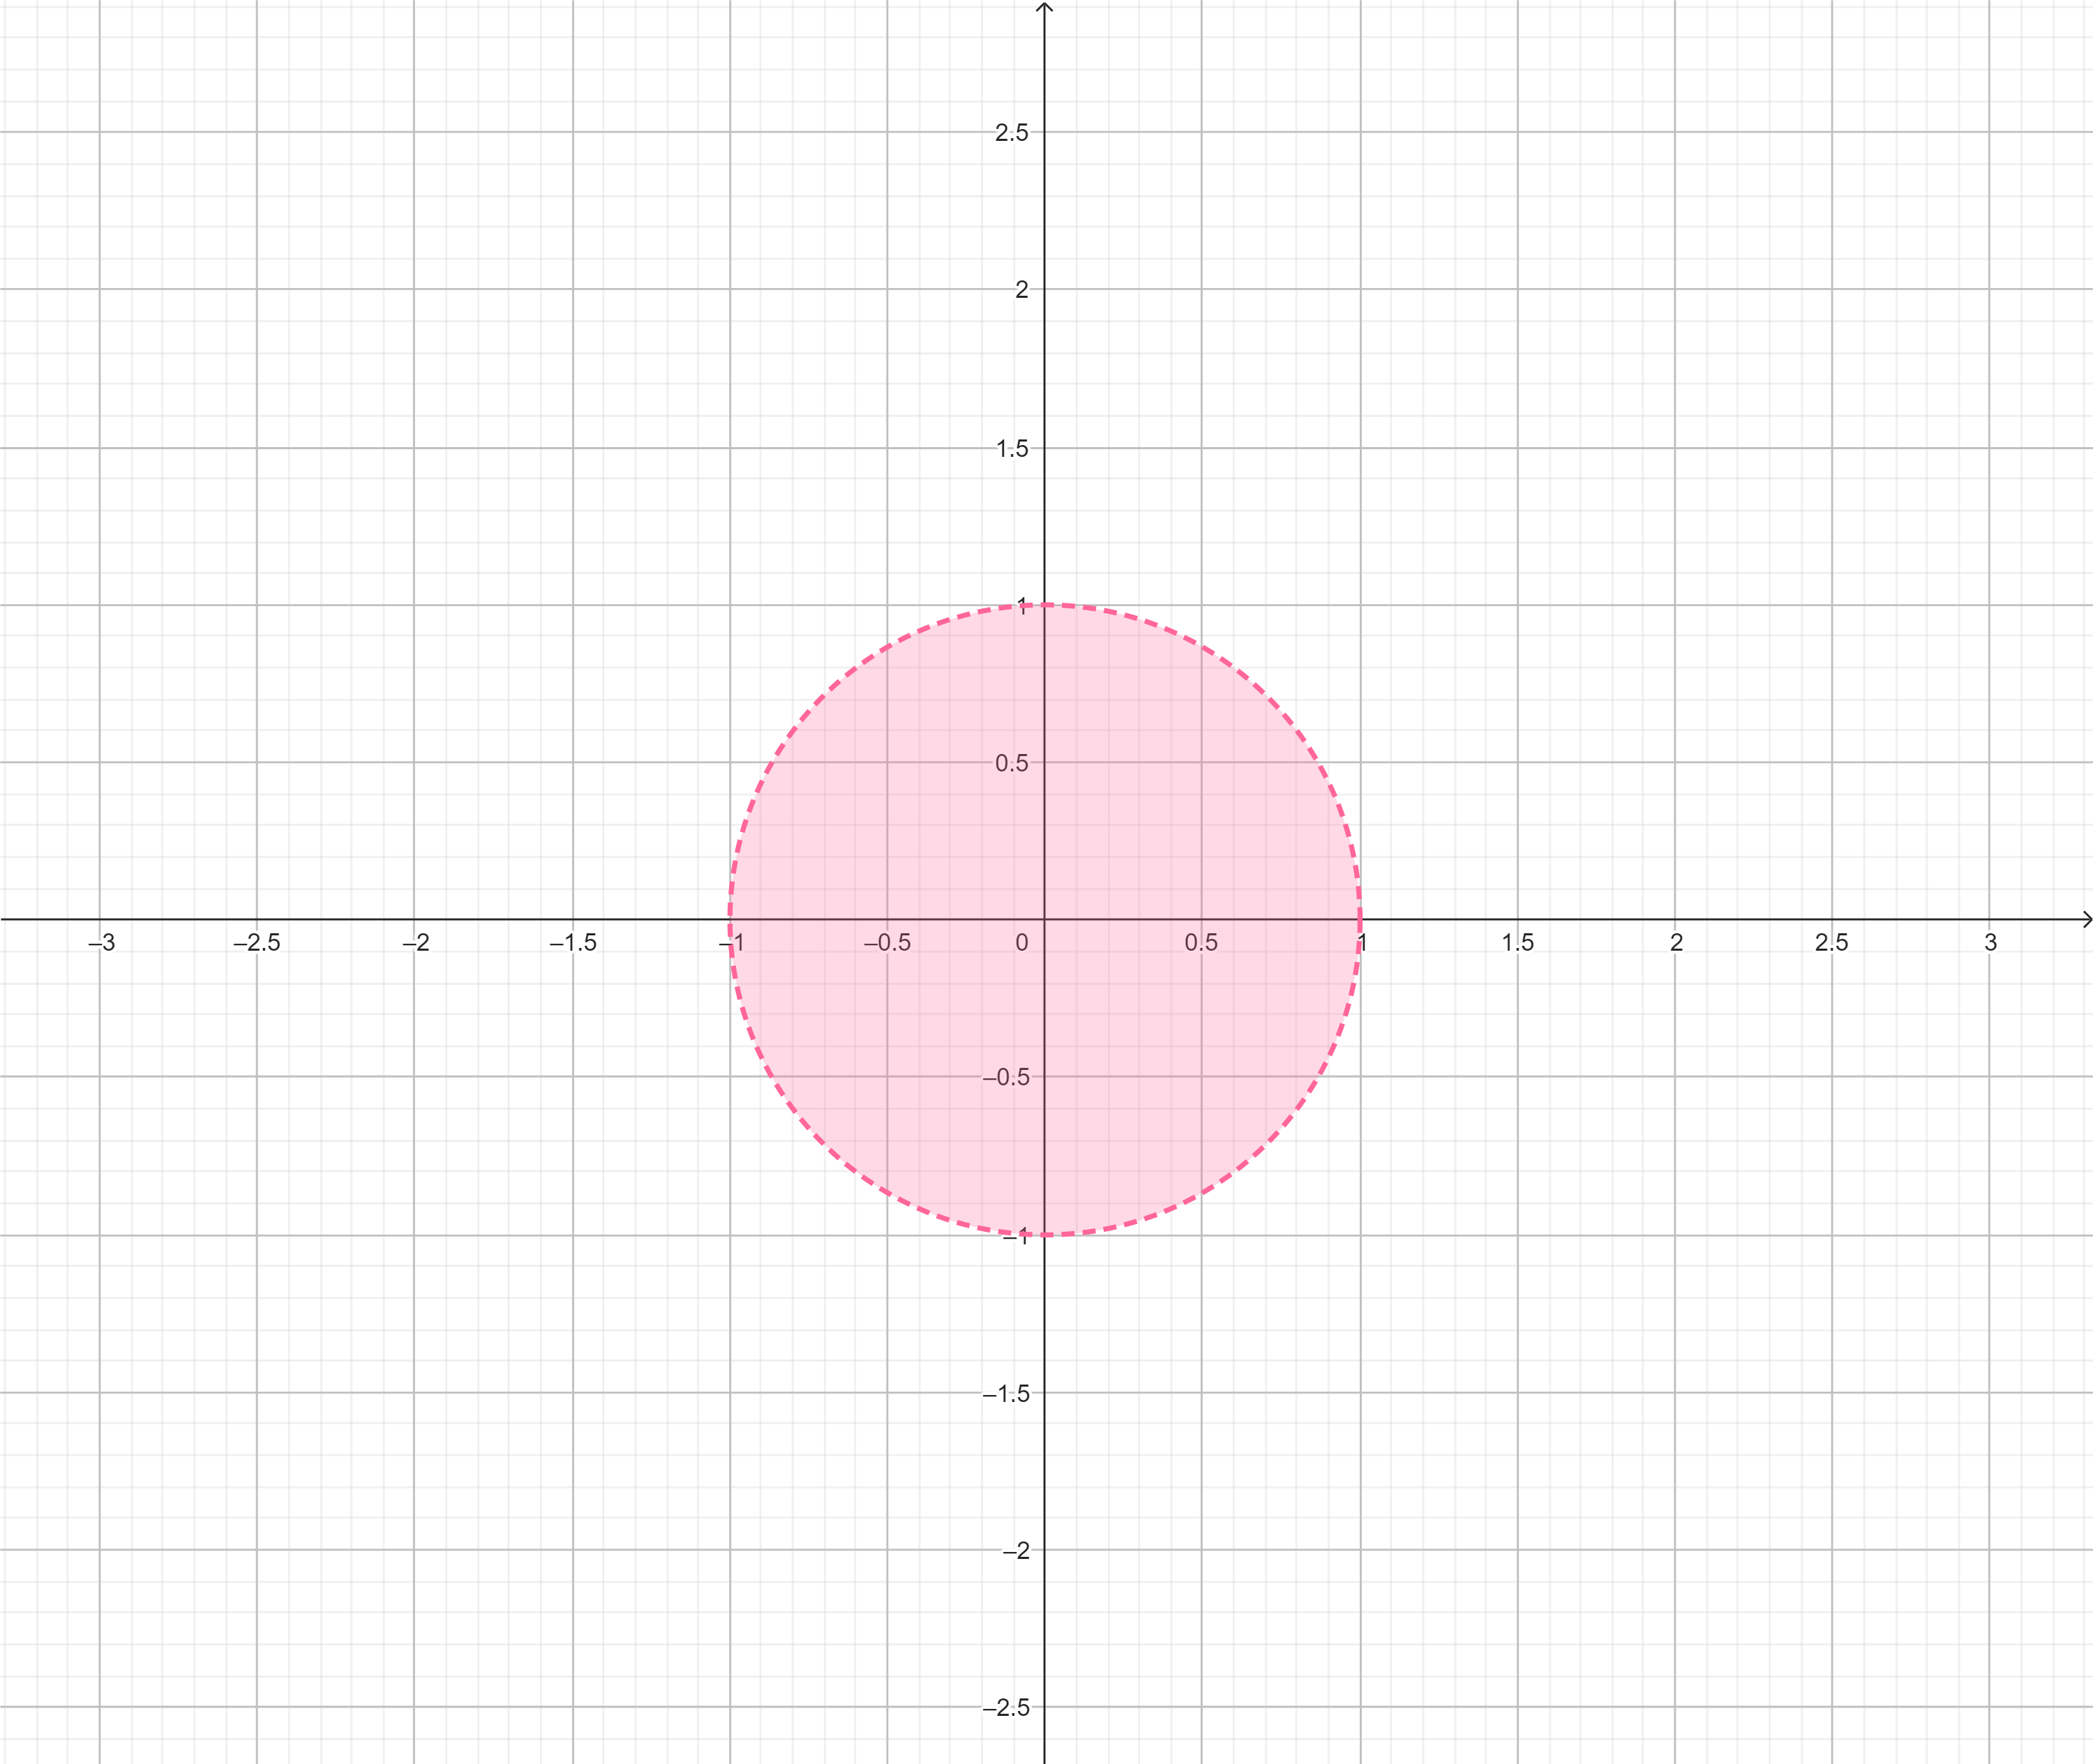
\includegraphics[scale=0.20] {graph1}
    	\caption{\label{fig:1} Open ball $B((0,0), 1) $ in $\alpha$ metric }
    \end{figure}
    
    
    \begin{figure}
    	\centering
    	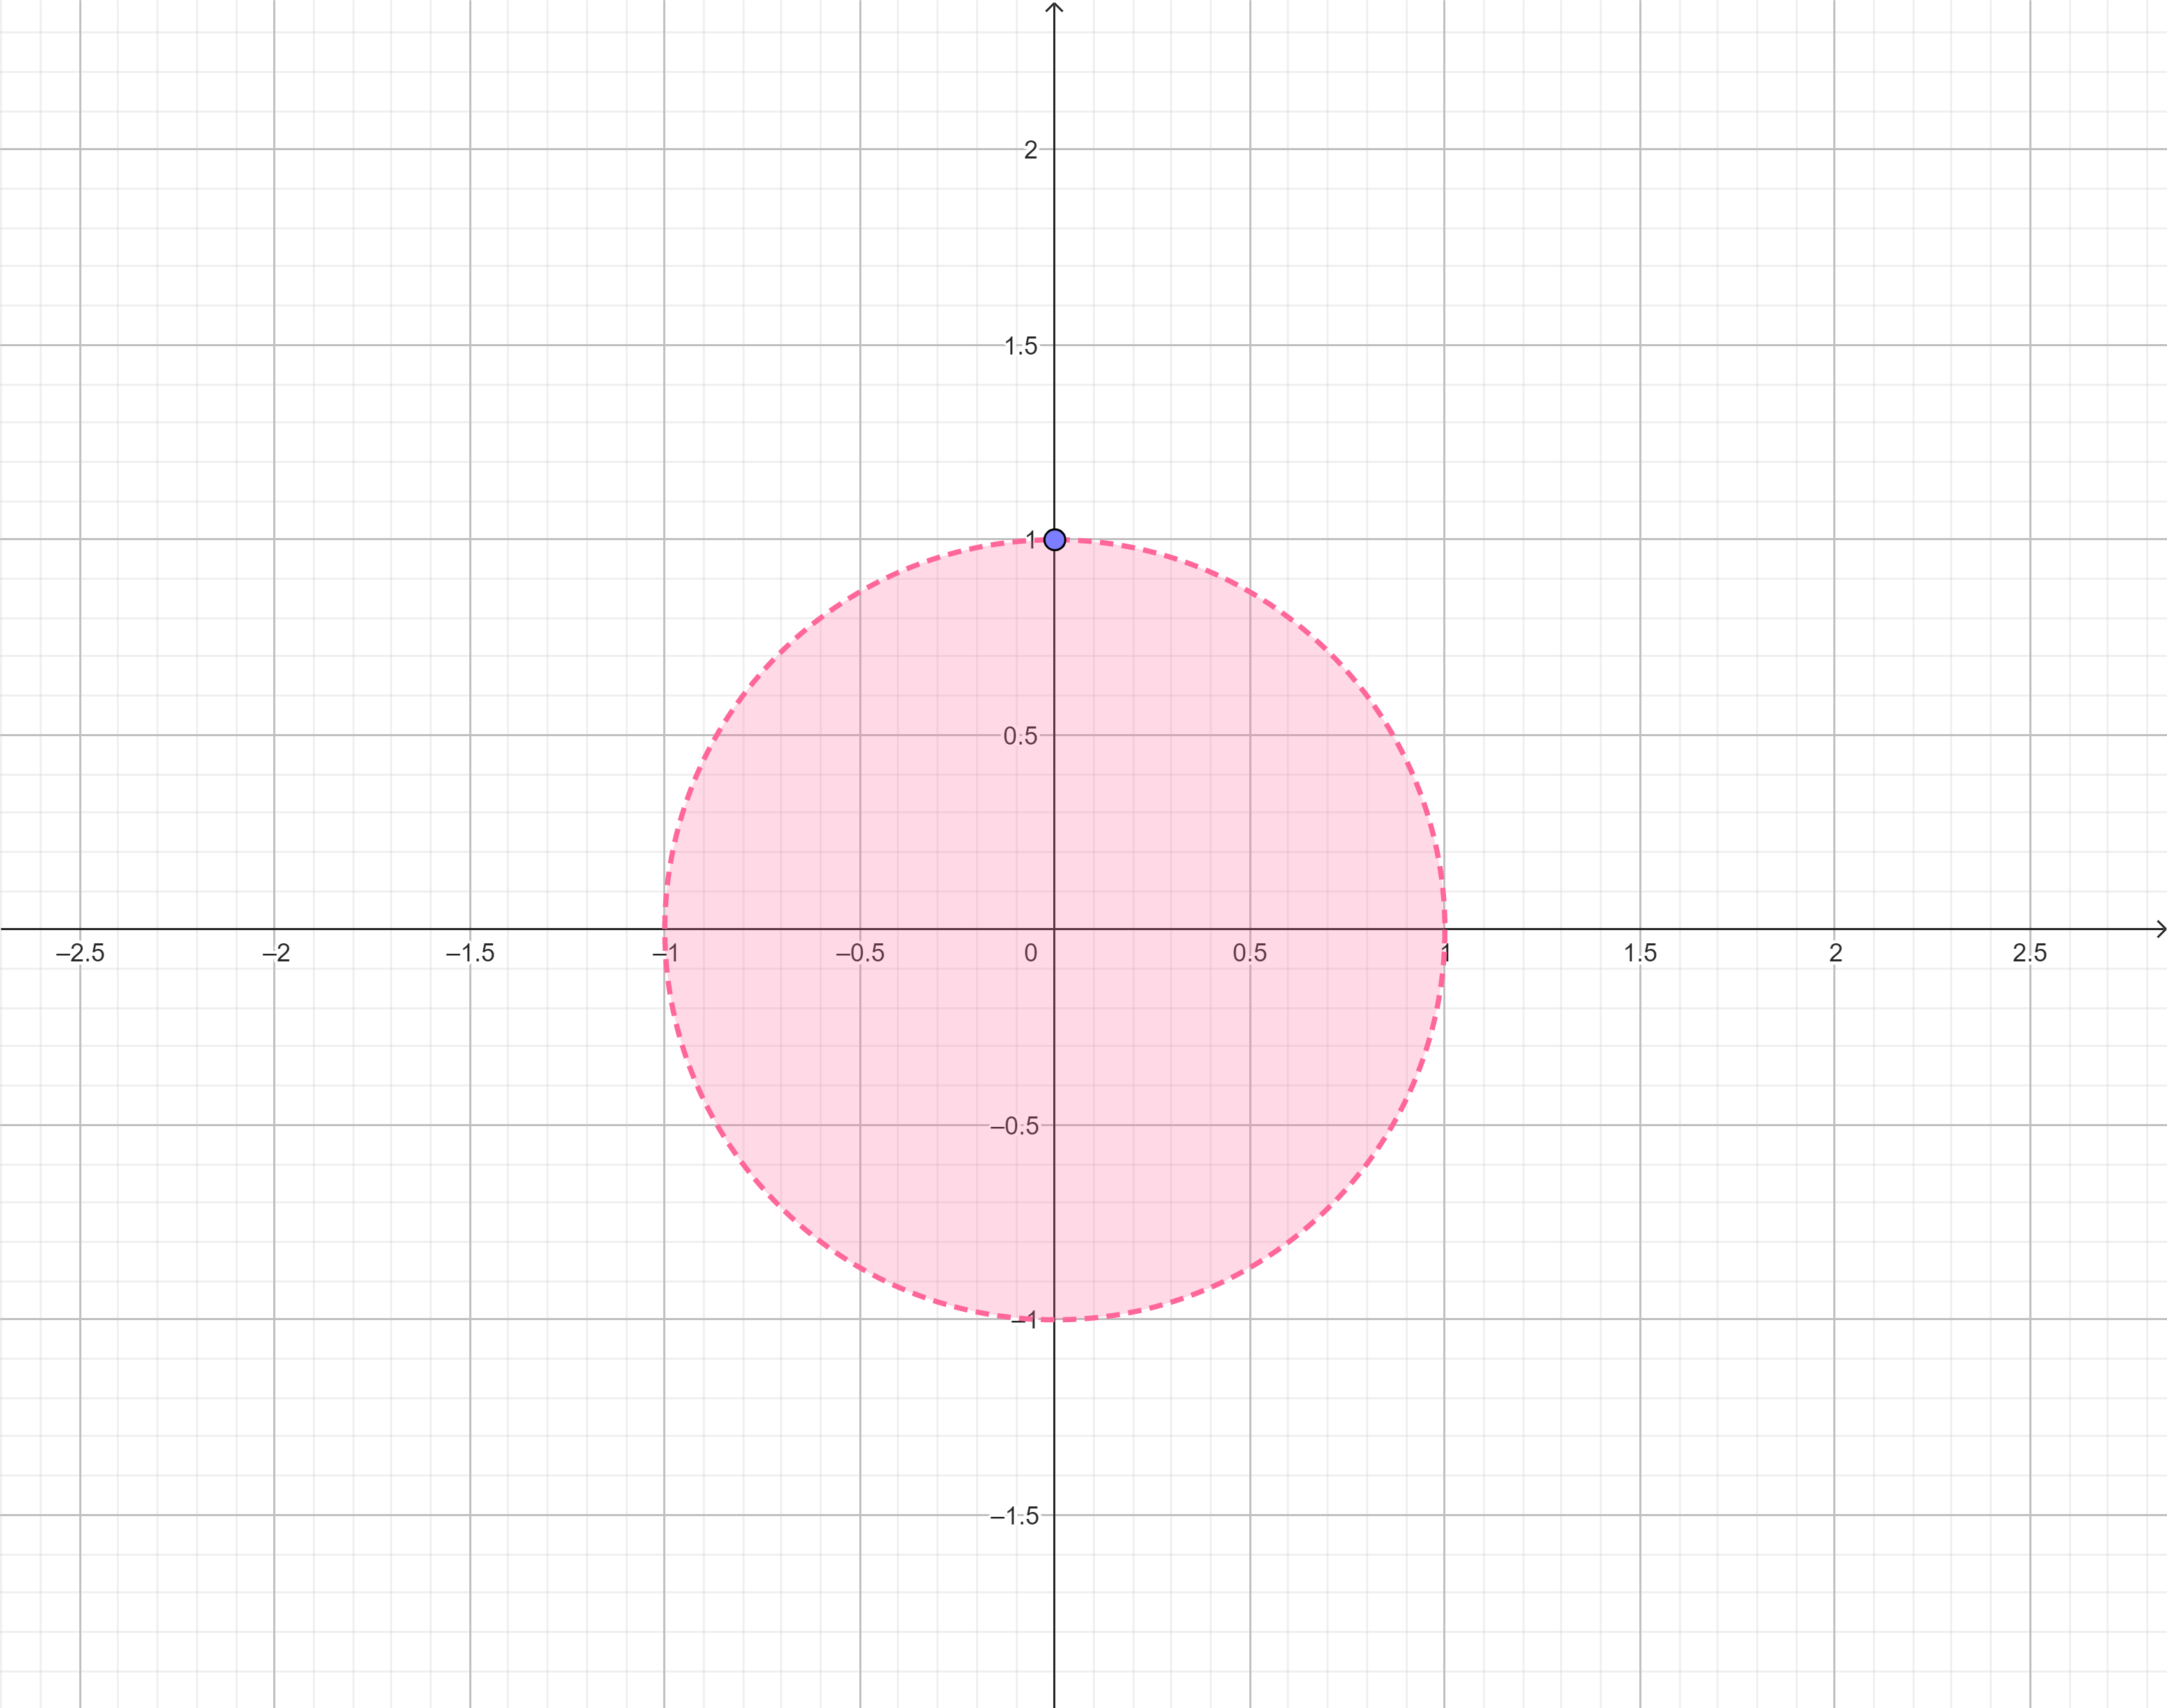
\includegraphics[scale=0.20] {graph2}
    	\caption{\label{fig:2} Open ball $B((0,1), 2) $ in $\alpha$ metric }
    \end{figure}

 \begin{figure}
	\centering
	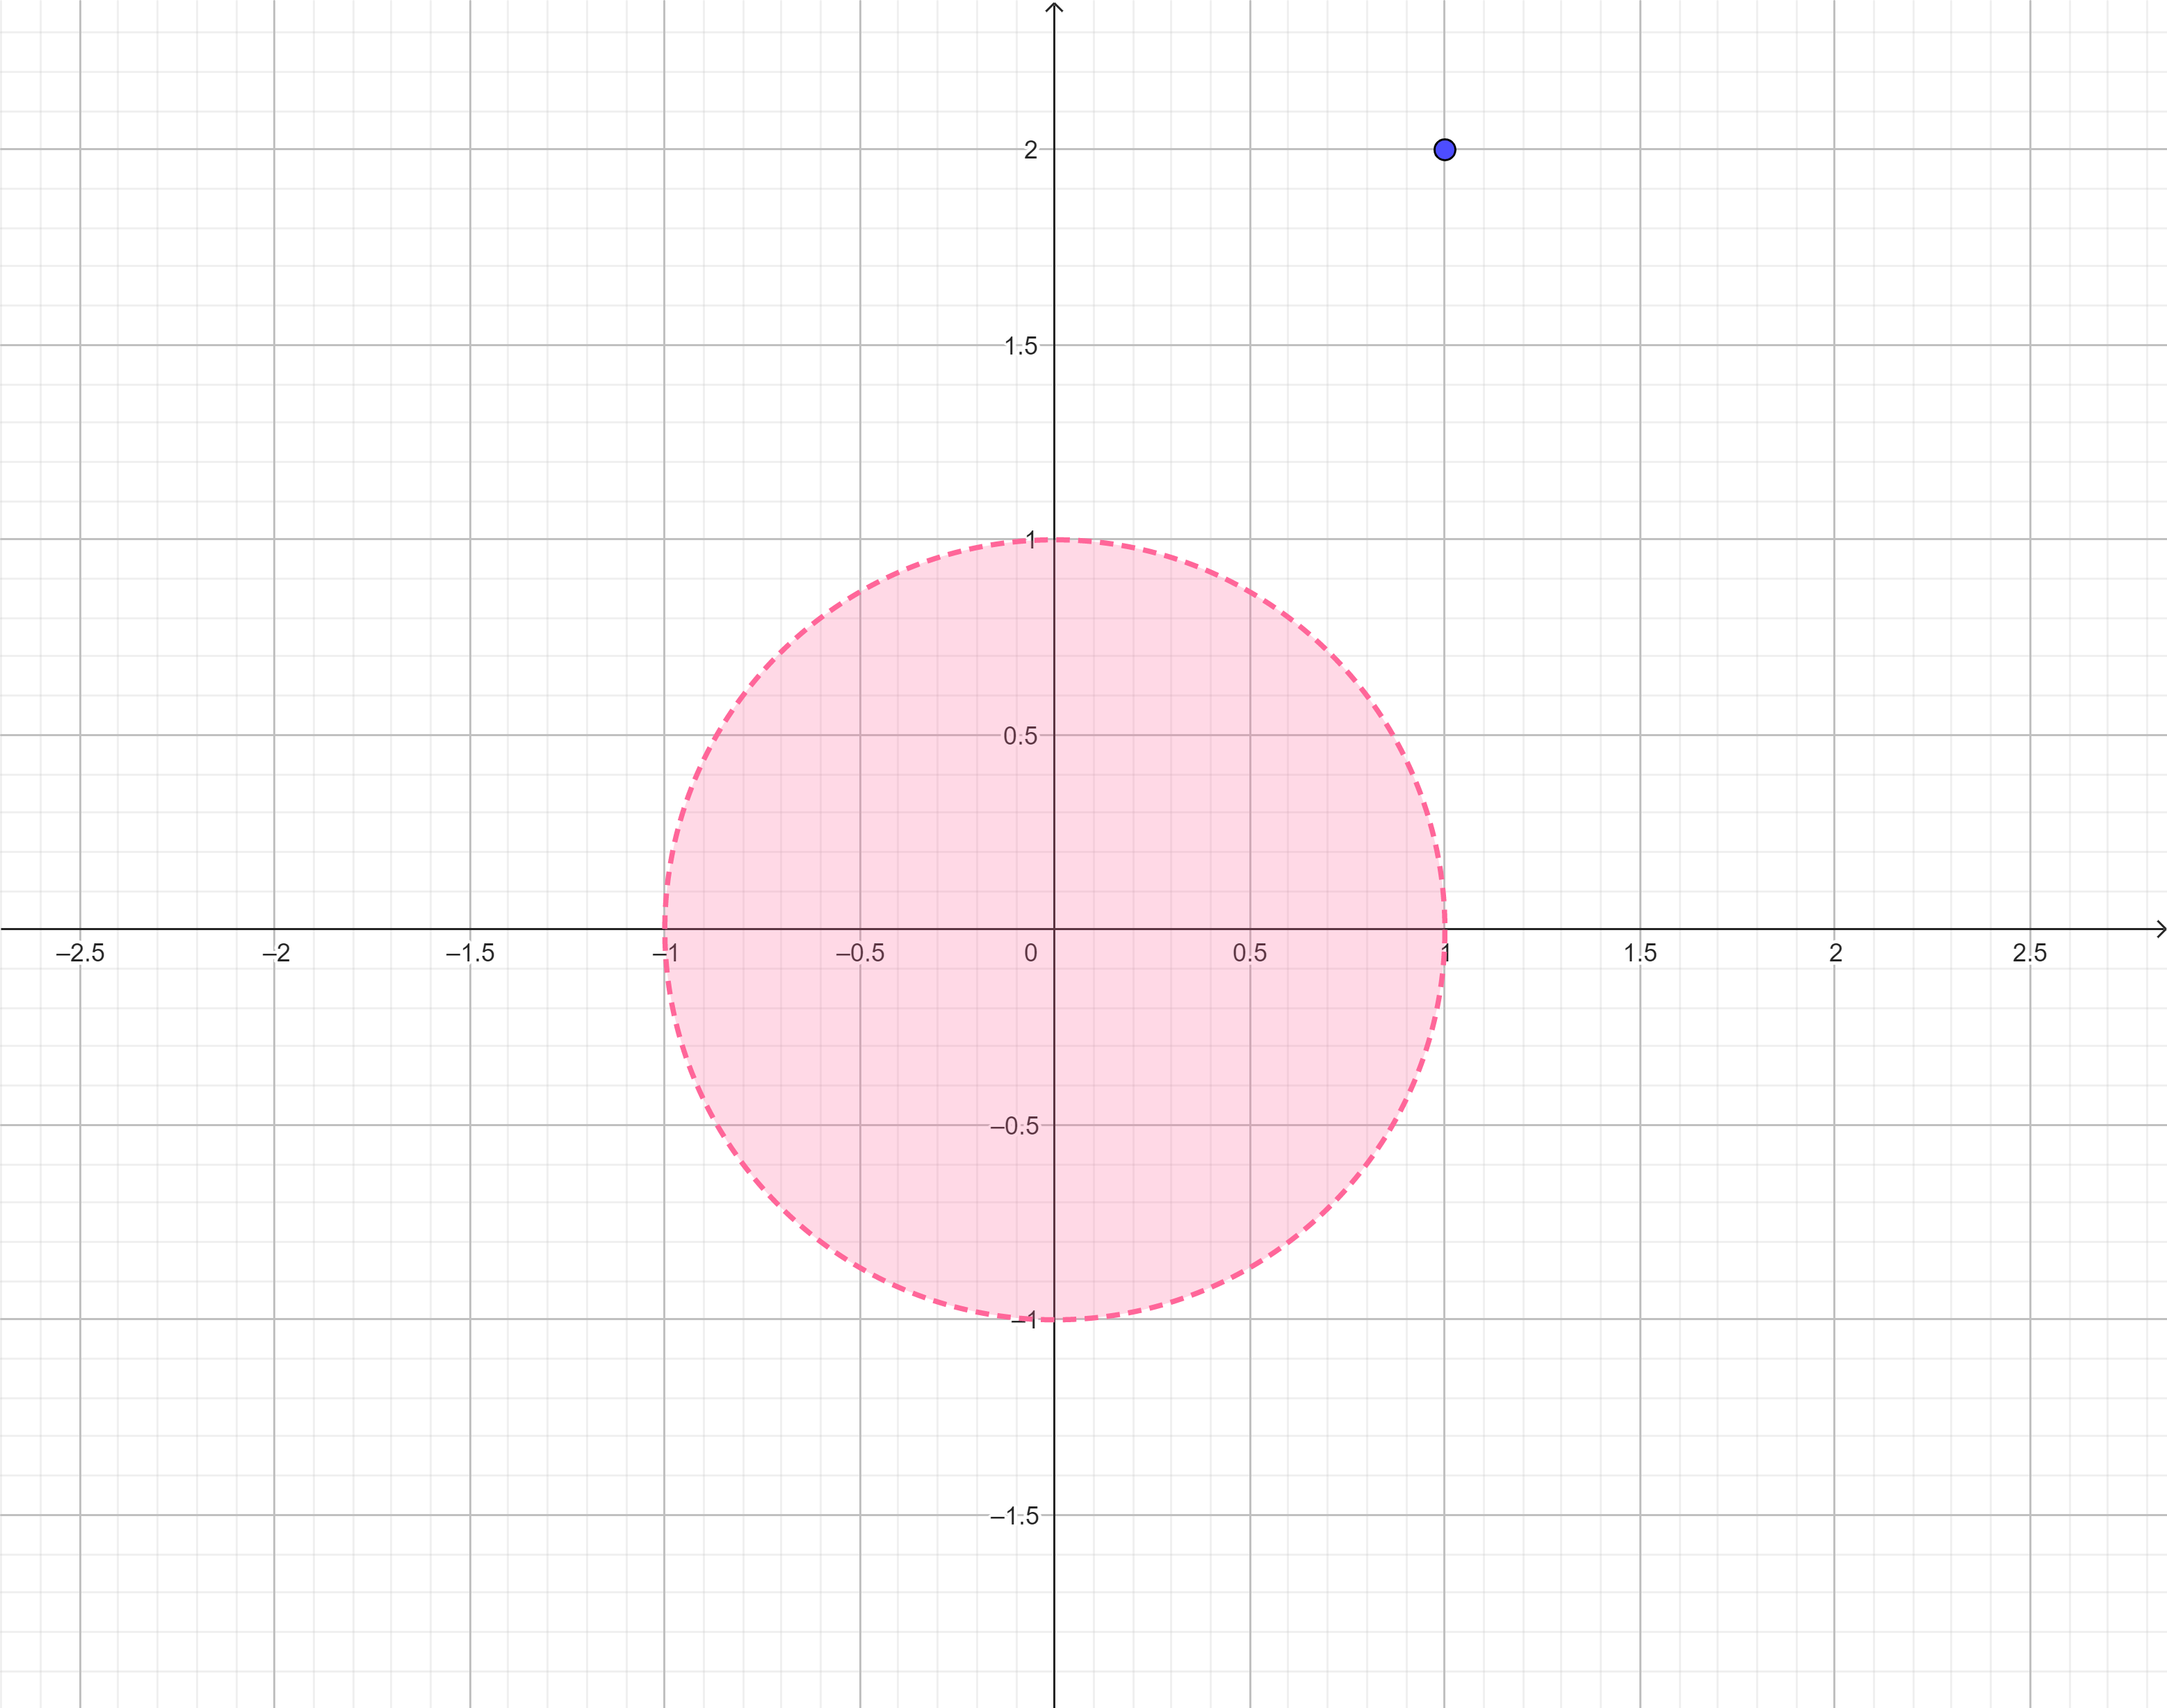
\includegraphics[scale=0.20] {graph3}
	\caption{\label{fig:2} Open ball $B((1,2), 1+\sqrt{5}) $ in $\alpha$ metric }
\end{figure}

	 


    \begin{align*} B((0,0), 1) &= \{(x_{1}, x_{2}) \in \mathbb{R}; \ \alpha((0,0),(x_{1}, x_{2}))<1\} \\
    &= \{(x_{1}, x_{2}) \in \mathbb{R}; \ x_{1} = 0 \land x_{2} = 0 \land 0 < 1 \} \cup \{(x_{1}, x_{2}) \in \mathbb{R}; \ x_{1} \neq 0 \lor x_{2} \neq 0 \land \sqrt{x_{1}^2 + x_{2}^2} < 1 \\
    &= \{(0,0) \} \cup \{(x_{1}, x_{2}) \in \mathbb{R}; \ x_{1} \neq 0 \lor x_{2} \neq 0 \land x_{1}^2 + x_{2}^2 < 1\} \\
     &= \{(x_{1}, x_{2}) \in \mathbb{R}; \ x_{1}^2 + x_{2}^2 < 1\} 
	\end{align*}
    
    \begin{align*} B((0,1), 2) &= \{(x_{1}, x_{2}) \in \mathbb{R}; \ \alpha((0,1),(x_{1}, x_{2}))<2\} \\
    	&= \{(x_{1}, x_{2}) \in \mathbb{R}; \ x_{1} = 0 \land x_{2} = 1 \land 0 < 2 \} \cup \{(x_{1}, x_{2}) \in \mathbb{R}; \ x_{1} \neq 0 \lor x_{2} \neq 1 \land \sqrt{0^2 + 1^2}  \\
    	&+ \sqrt{x_{1}^2 + x_{2}^2} < 2 \}\\
    	&= \{(0,1) \} \cup \{(x_{1}, x_{2}) \in \mathbb{R}; \ x_{1} \neq 0 \lor x_{2} \neq 1 \land \sqrt{1} + \sqrt{x_{1}^2 + x_{2}^2} < 2\} \\
    	&= \{(0,1) \} \cup \{(x_{1}, x_{2}) \in \mathbb{R}; \ \sqrt{x_{1}^2 + x_{2}^2} < 1\} \\
    	&= \{(0,1) \} \cup \{(x_{1}, x_{2}) \in \mathbb{R}; \ x_{1}^2 + x_{2}^2 < 1\}	
    \end{align*}

	\begin{align*} B((1,2), 1+\sqrt{5}) &= \{(x_{1}, x_{2}) \in \mathbb{R}; \ \alpha((1,2),(x_{1}, x_{2}))<1+\sqrt{5}\} \\
		&= \{(x_{1}, x_{2}) \in \mathbb{R}; \ x_{1} = 1 \land x_{2} = 2 \land 0 < 1 + \sqrt{5} \} \cup \{(x_{1}, x_{2}) \in \mathbb{R}; \ x_{1} \neq 1 \lor x_{2} \neq 2   \\
		&\land \sqrt{1^2 + 2^2} + \sqrt{x_{1}^2 + x_{2}^2} < 1 + \sqrt{5} \}\\
		&= \{(1,2) \} \cup \{(x_{1}, x_{2}) \in \mathbb{R}; \ x_{1} \neq 1 \lor x_{2} \neq 2 \land \sqrt{5} + \sqrt{x_{1}^2 + x_{2}^2} < 1 + \sqrt{5}\} \\
		&= \{(1,2) \} \cup \{(x_{1}, x_{2}) \in \mathbb{R}; \ \sqrt{x_{1}^2 + x_{2}^2} < 1\} \\
		&= \{(1,2) \} \cup \{(x_{1}, x_{2}) \in \mathbb{R}; \ x_{1}^2 + x_{2}^2 < 1\}	
	\end{align*}

	\textbf{(c)} I drew the open balls $B((0,0), 1)$, $B((0,1), 2)$ and $B((2,2), \sqrt{2})$ in $\beta$ metric. The drawings can be seen on Figures 4,5 and 6. The calculations I made were: 
	
	\begin{figure}
		\centering
		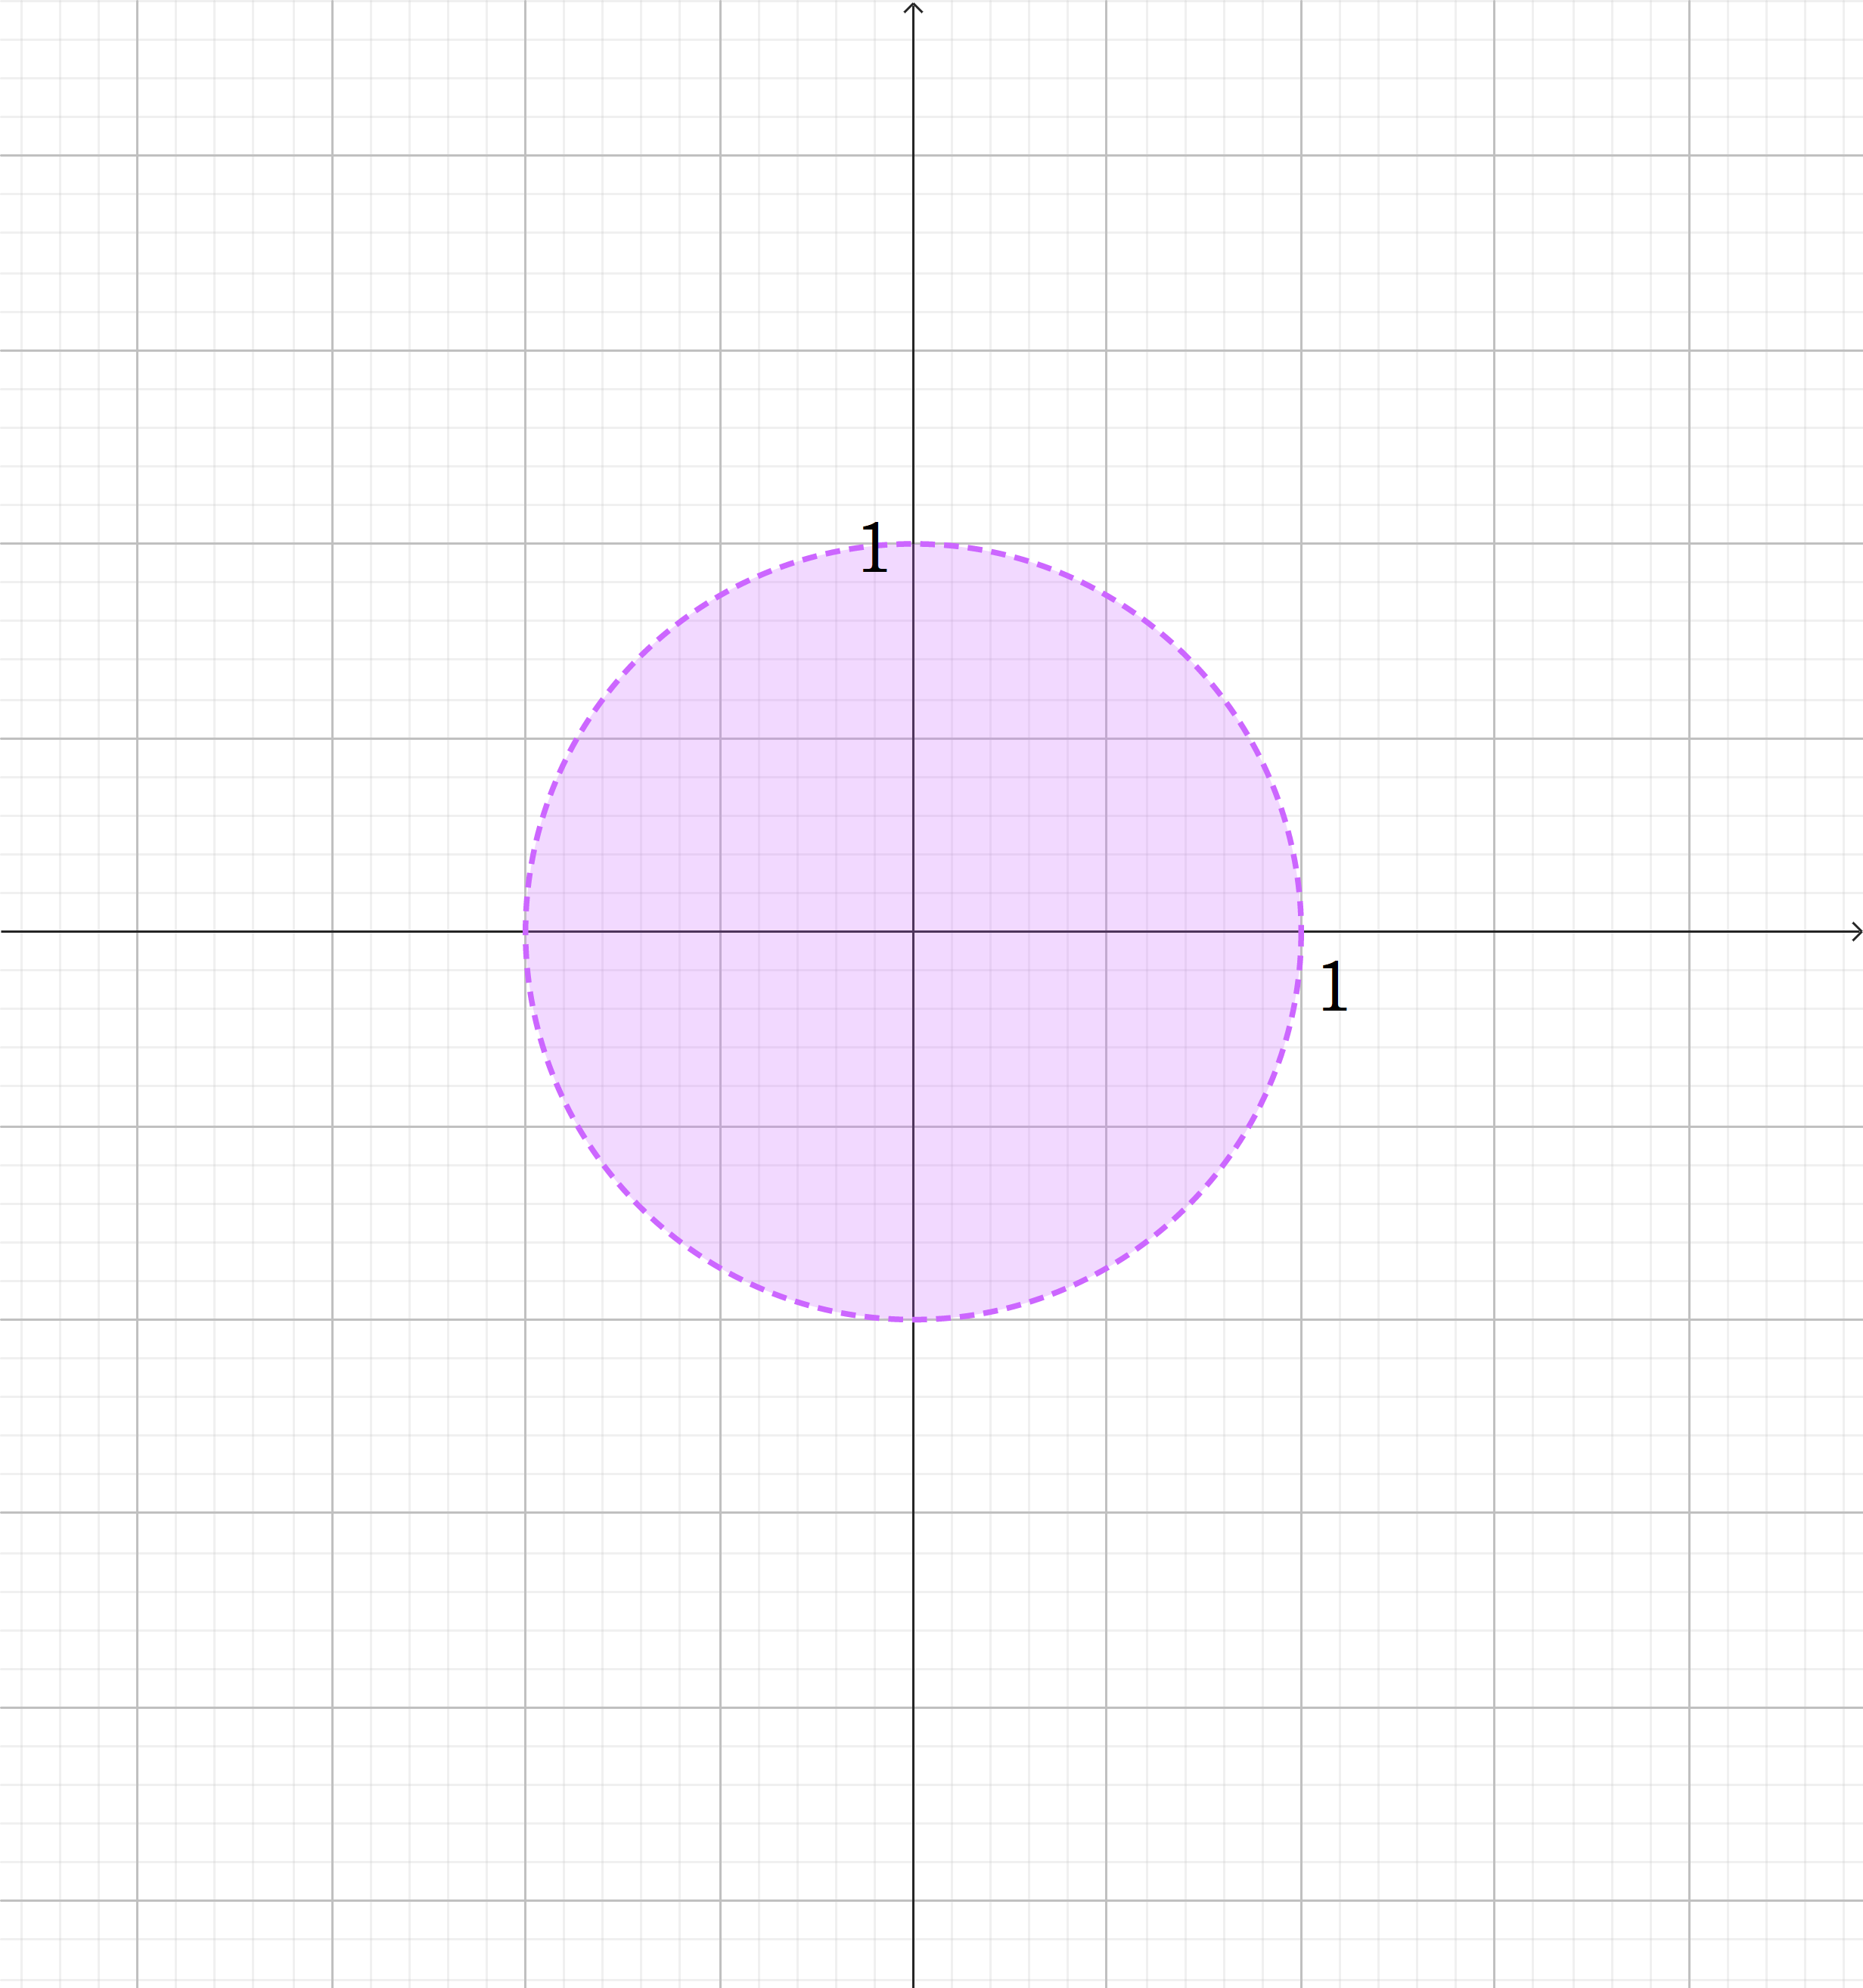
\includegraphics[scale=0.20] {graph4}
		\caption{\label{fig:4} Open ball $B((0,0), 1) $ in $\beta$ metric }
	\end{figure}
	
	
	\begin{figure}
		\centering
		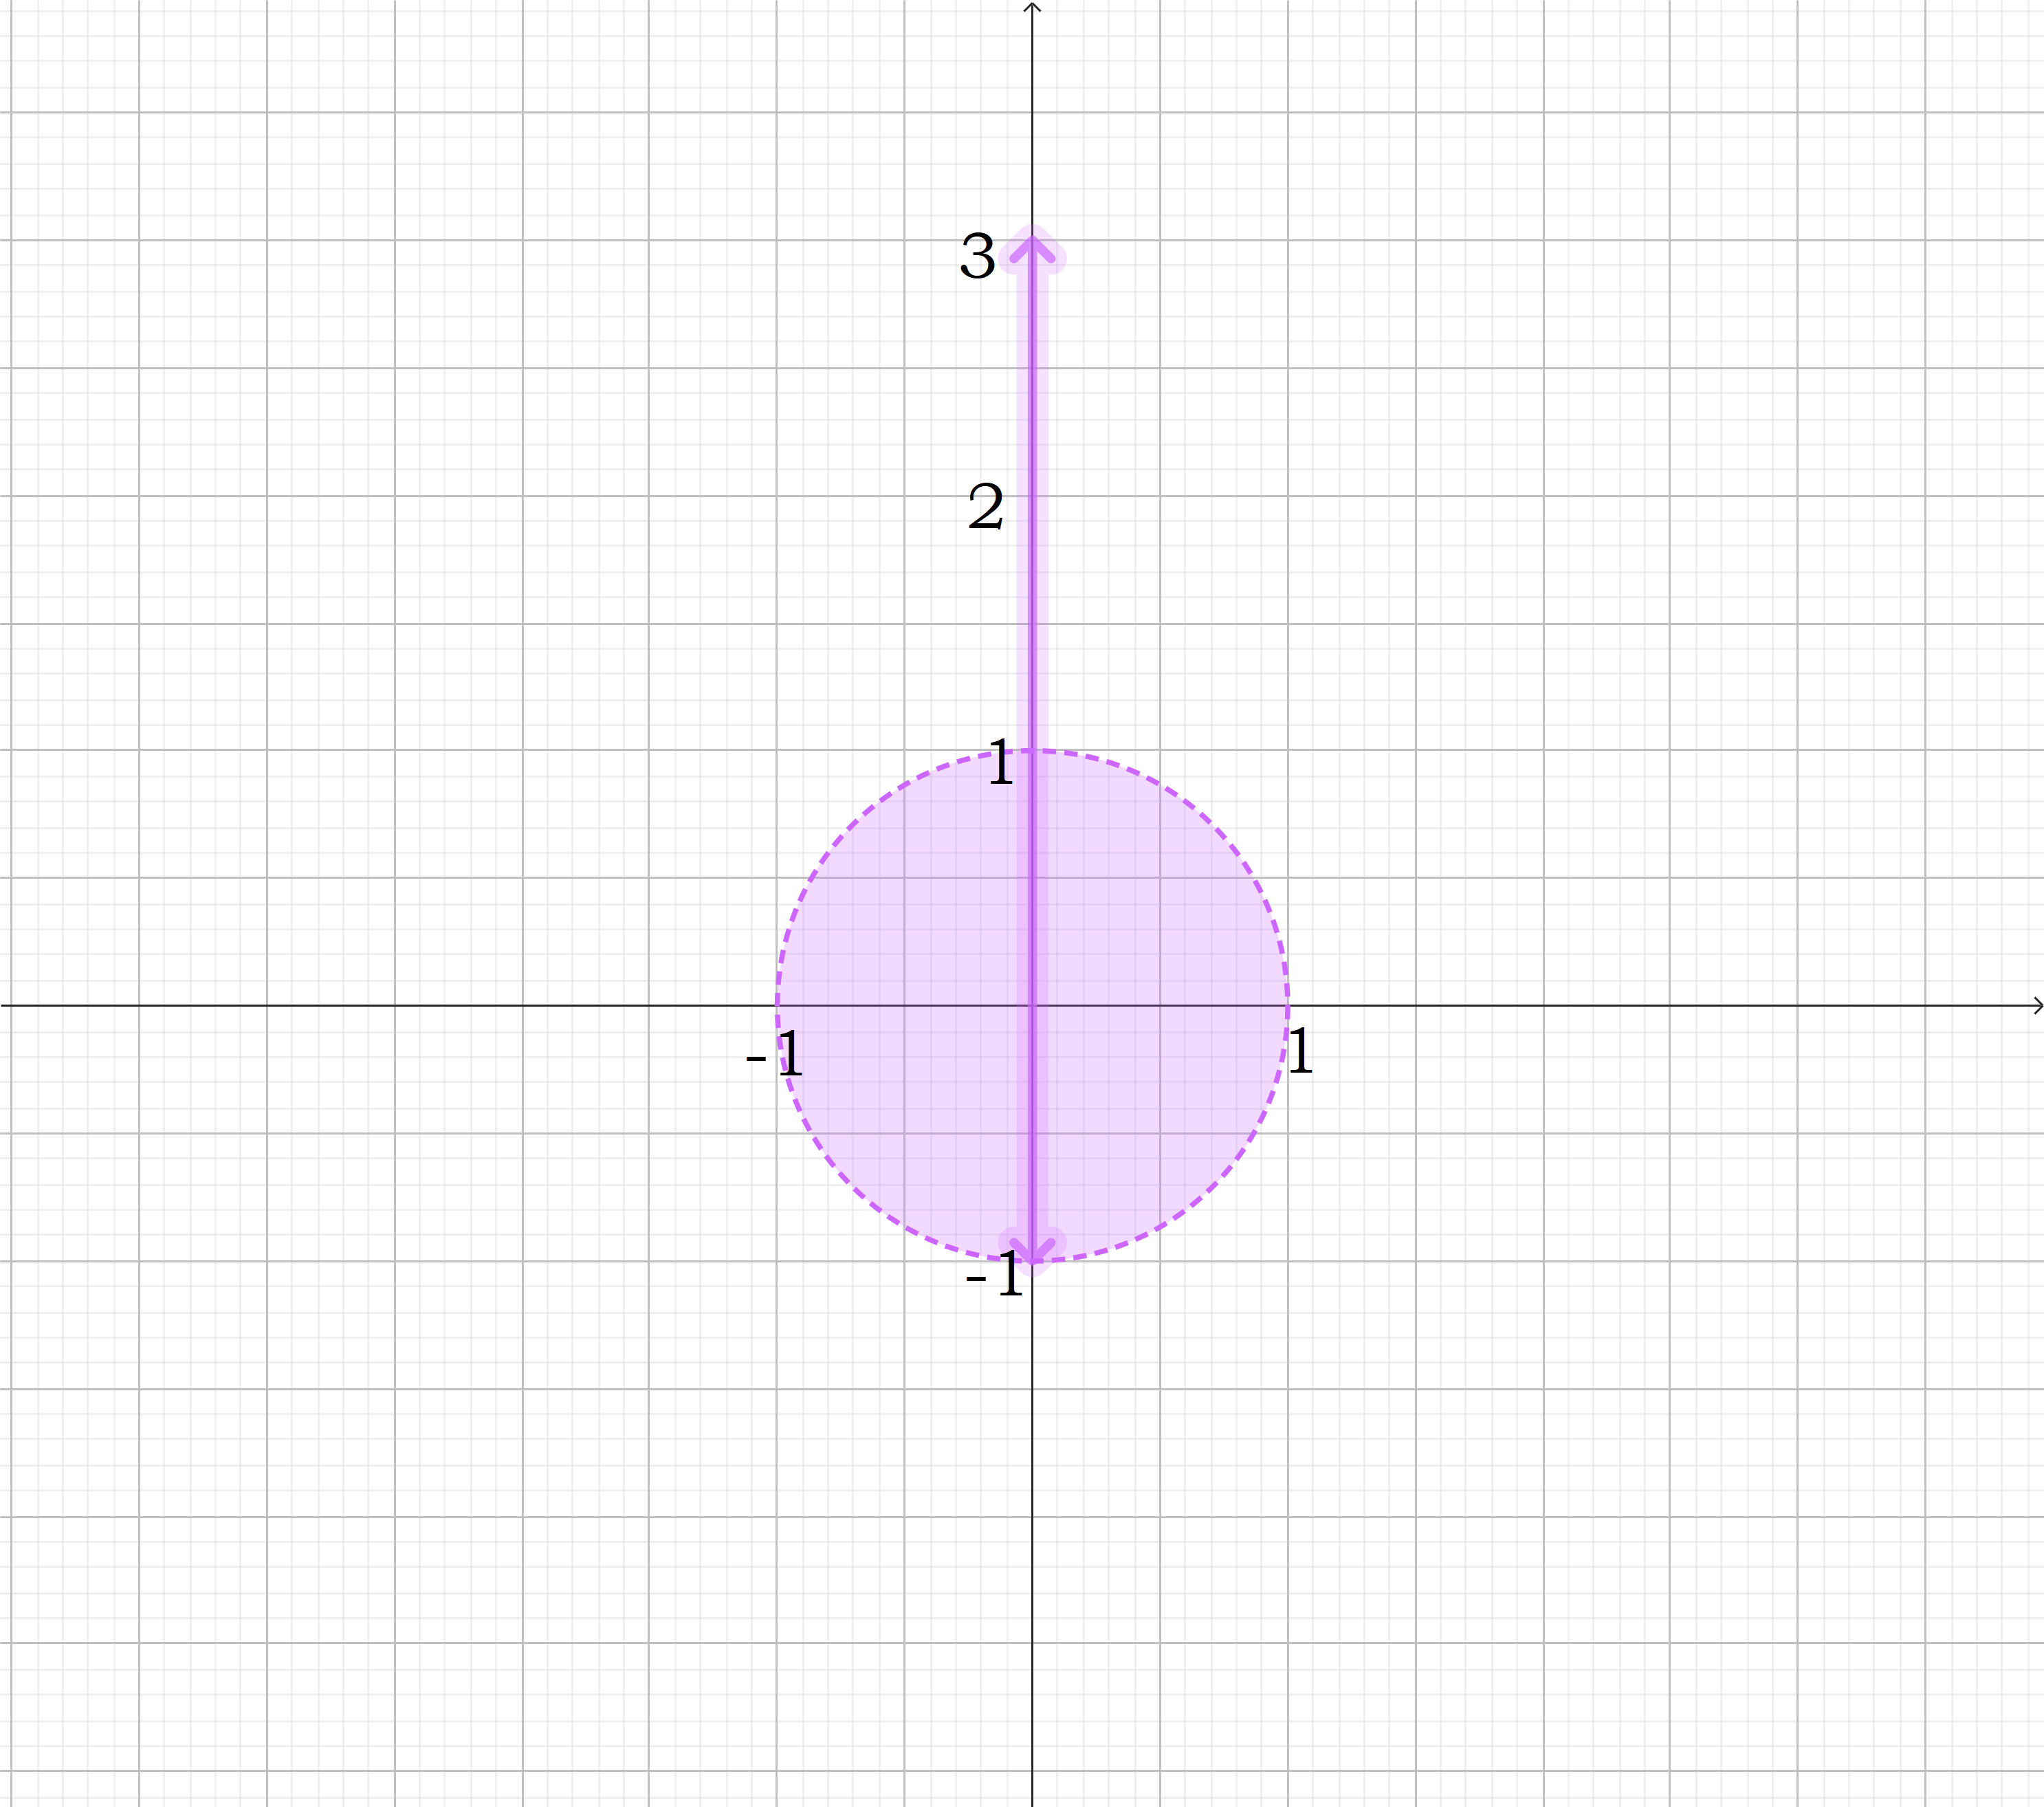
\includegraphics[scale=0.20] {graph5}
		\caption{\label{fig:5} Open ball $B((0,1), 2) $ in $\beta$ metric }
	\end{figure}
	
	\begin{figure}
		\centering
		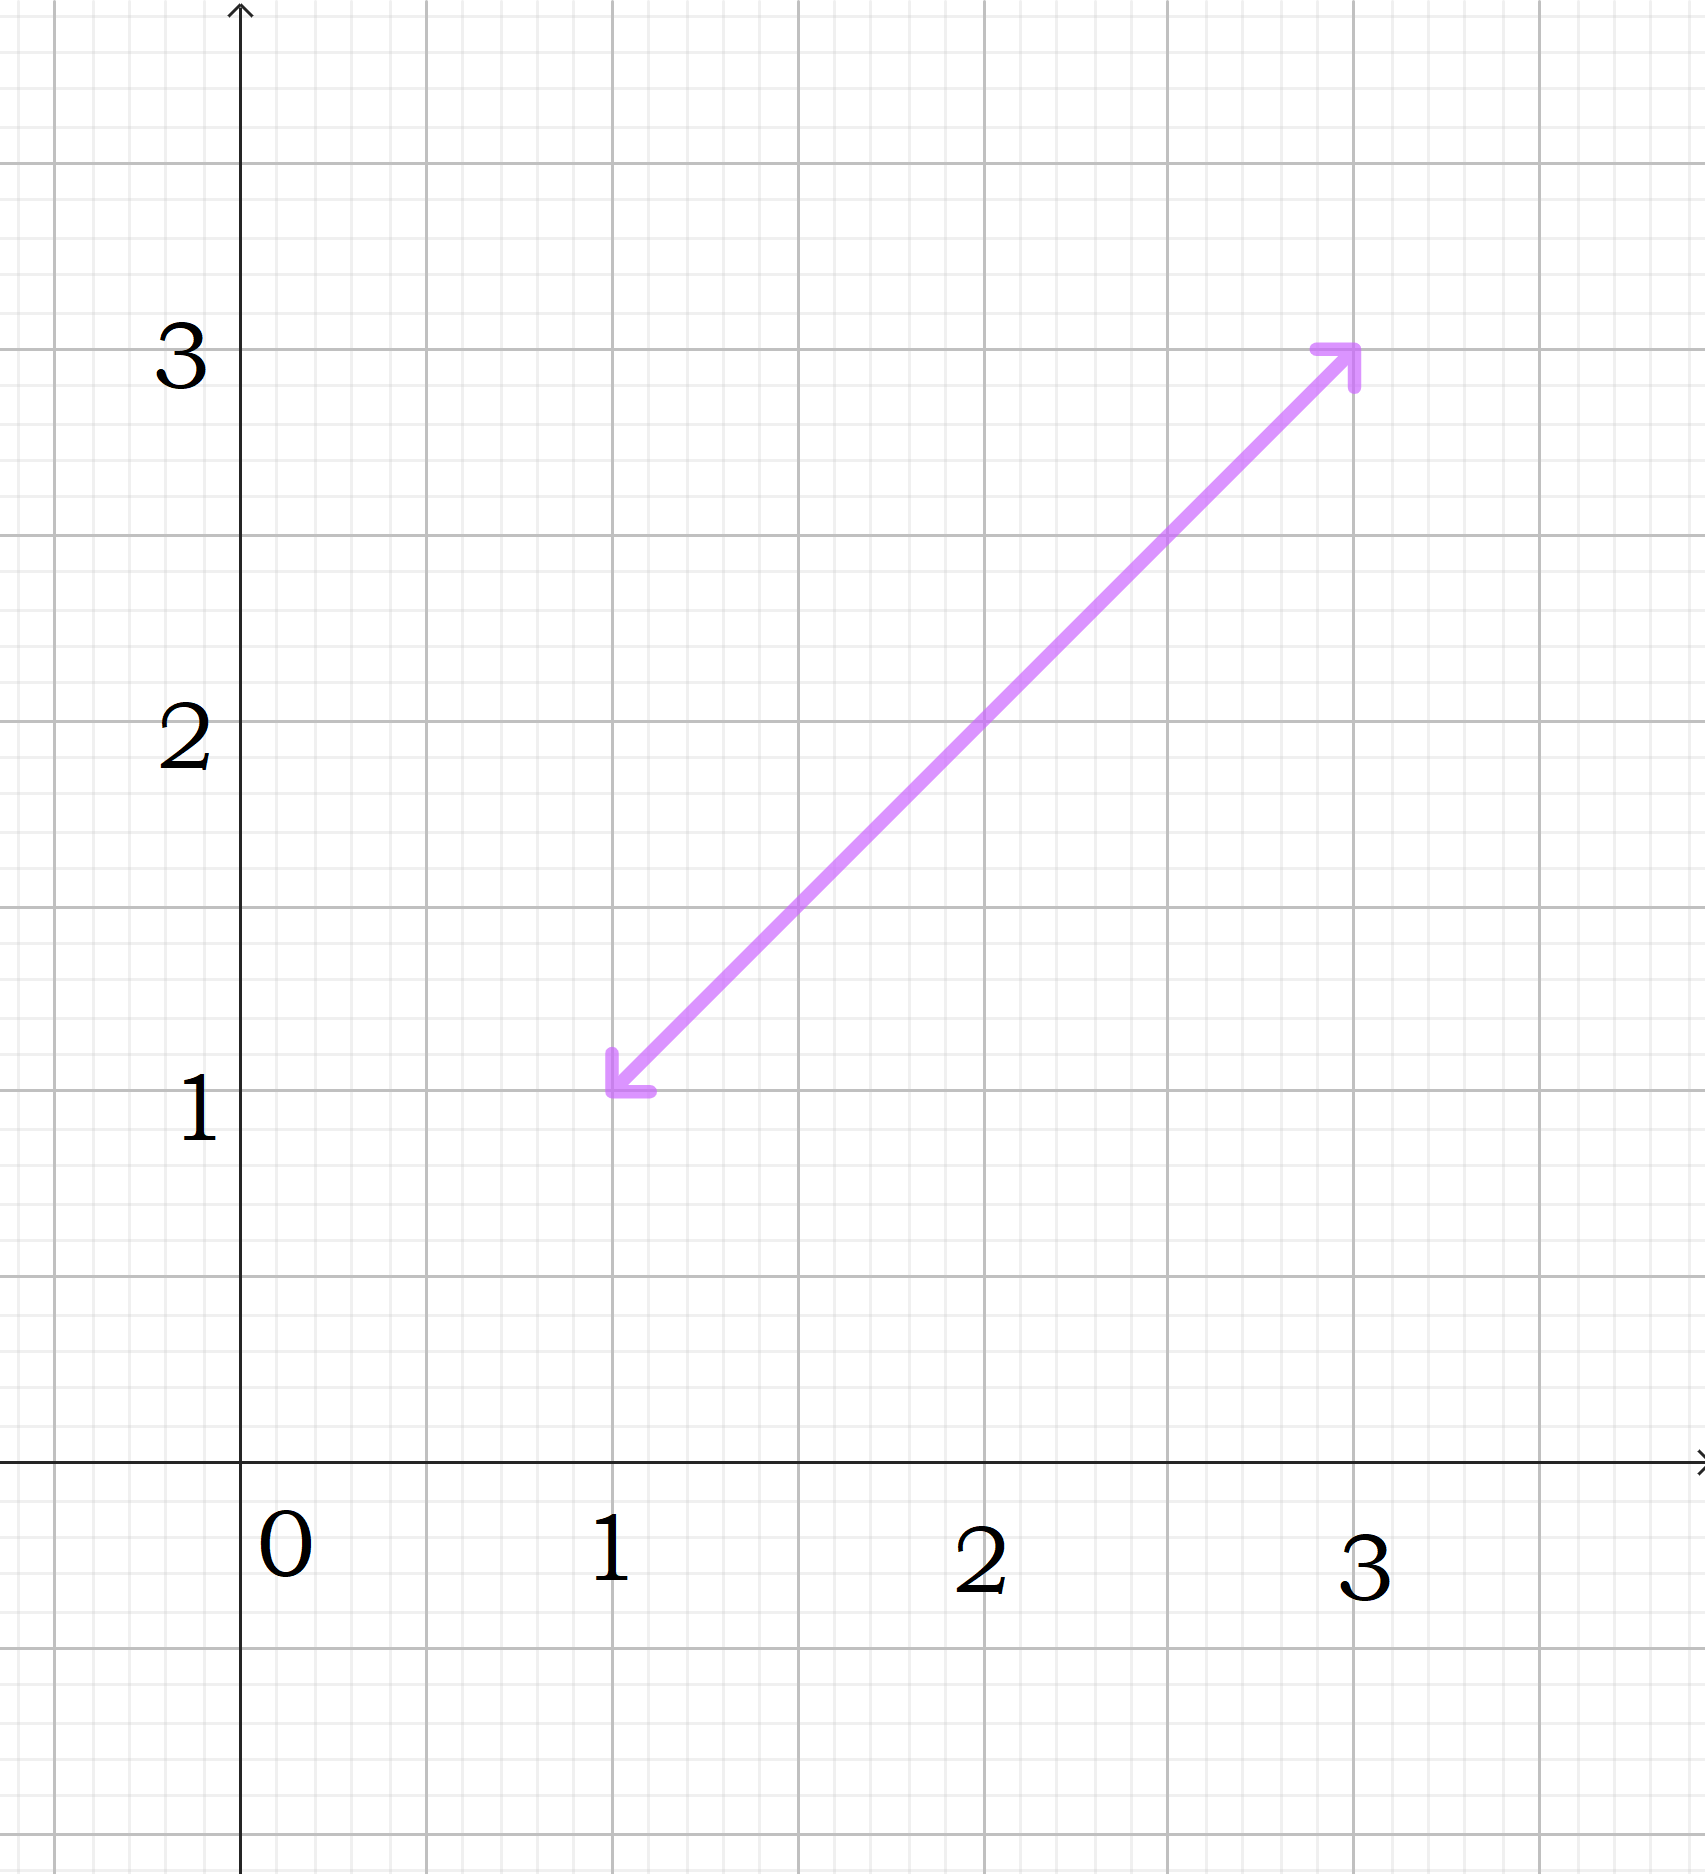
\includegraphics[scale=0.20] {graph6}
		\caption{\label{fig:6} Open ball $B((1,2), \sqrt{2}) $ in $\beta$ metric }
	\end{figure}
	
	\begin{align*} B((0,0), 1) &= \{(x_{1}, x_{2}) \in \mathbb{R}; \ \beta((0,0),(x_{1}, x_{2}))<1\} \\
		&= \{(x_{1}, x_{2}) \in \mathbb{R}; \ 0 \cdot x_{2} = 0 \cdot x_{1} \land  \sqrt{(0-x_{1})^2 + (0-x_{2})^2} < 1 \} \ \cup \\ 
		&\{(x_{1}, x_{2}) \in \mathbb{R}; \ 0 \cdot x_{2} \neq 0 \cdot x_{1} \land  \sqrt{0^2 + 0^2} + \sqrt{x_{1}^2 + x_{2}^2} < 1 \\
		&= \{(x_{1}, x_{2}) \in \mathbb{R}; \  \sqrt{(-x_{1})^2 + (-x_{2})^2} < 1 \} \cup \emptyset \\
		&= \{(x_{1}, x_{2}) \in \mathbb{R}; \ x_{1}^2 + x_{2}^2 < 1\} 
	\end{align*}

	\begin{align*} B((0,1), 2) &= \{(x_{1}, x_{2}) \in \mathbb{R}; \ \beta((0,1),(x_{1}, x_{2}))<2\} \\
		&= \{(x_{1}, x_{2}) \in \mathbb{R}; \ 0 \cdot x_{2} = 1 \cdot x_{1} \land  \sqrt{(0-x_{1})^2 + (1-x_{2})^2} < 2 \} \ \cup \\ 
		&\{(x_{1}, x_{2}) \in \mathbb{R}; \ 0 \cdot x_{2} \neq 1 \cdot x_{1} \land  \sqrt{0^2 + 1^2} + \sqrt{x_{1}^2 + x_{2}^2} < 2 \} \\
		&=\{(x_{1}, x_{2}) \in \mathbb{R}; \ x_{1} = 0 \land  \sqrt{(1-x_{2})^2} < 2 \} \ \cup 
		\{(x_{1}, x_{2}) \in \mathbb{R}; \ x_{1} \neq 0 \land  \sqrt{1} + \sqrt{x_{1}^2 + x_{2}^2} < 2 \} \\ 
		&=\{(x_{1}, x_{2}) \in \mathbb{R}; \ x_{1} = 0 \land  |1-x_{2}| < 2 \} \ \cup 
		\{(x_{1}, x_{2}) \in \mathbb{R}; \ x_{1} \neq 0 \land \sqrt{x_{1}^2 + x_{2}^2} < 1 \} \\ 
		&=\{(0, x_{2}) \in \mathbb{R}; |1-x_{2}| < 2 \} \ \cup 
		\{(x_{1}, x_{2}) \in \mathbb{R}; \ x_{1} \neq 0 \land x_{1}^2 + x_{2}^2 < 1 \}
	\end{align*}

	\begin{align*} B((2,2), \sqrt{2}) &= \{(x_{1}, x_{2}) \in \mathbb{R}; \ \beta((2,2),(x_{1}, x_{2}))<\sqrt{2}\} \\
		&= \{(x_{1}, x_{2}) \in \mathbb{R}; \ 2 \cdot x_{2} = 2 \cdot x_{1} \land  \sqrt{(2-x_{1})^2 + (2-x_{2})^2} < \sqrt{2} \} \ \cup \\ 
		&\{(x_{1}, x_{2}) \in \mathbb{R}; \ 2 \cdot x_{2} \neq 2 \cdot x_{1} \land  \sqrt{2^2 + 2^2} + \sqrt{x_{1}^2 + x_{2}^2} < \sqrt{2} \} \\
		&=\{(x_{1}, x_{2}) \in \mathbb{R}; \ \cdot x_{1} = x_{2} \land  \sqrt{2\cdot(2-x_{2})^2} < \sqrt{2} \} \\
		&\cup 
		\{(x_{1}, x_{2}) \in \mathbb{R}; \ x_{1} \neq x_{2} \land \sqrt{8} + \sqrt{x_{1}^2 + x_{2}^2} < \sqrt{2} \} \\ 
		&=\{(x_{1}, x_{1}) \in \mathbb{R}; \ |2-x_{1}| < 2 \} \ \cup \emptyset
	\end{align*}

	\textbf{(d)} I drew the open balls $B((0,0), 1)$, $B((0,1), 2)$ and $B((2,2), \sqrt{2})$ in $\gamma$ metric. The drawings can be seen on Figures 7,8 and 9. The calculations I made were: 
	
		\begin{figure}
		\centering
		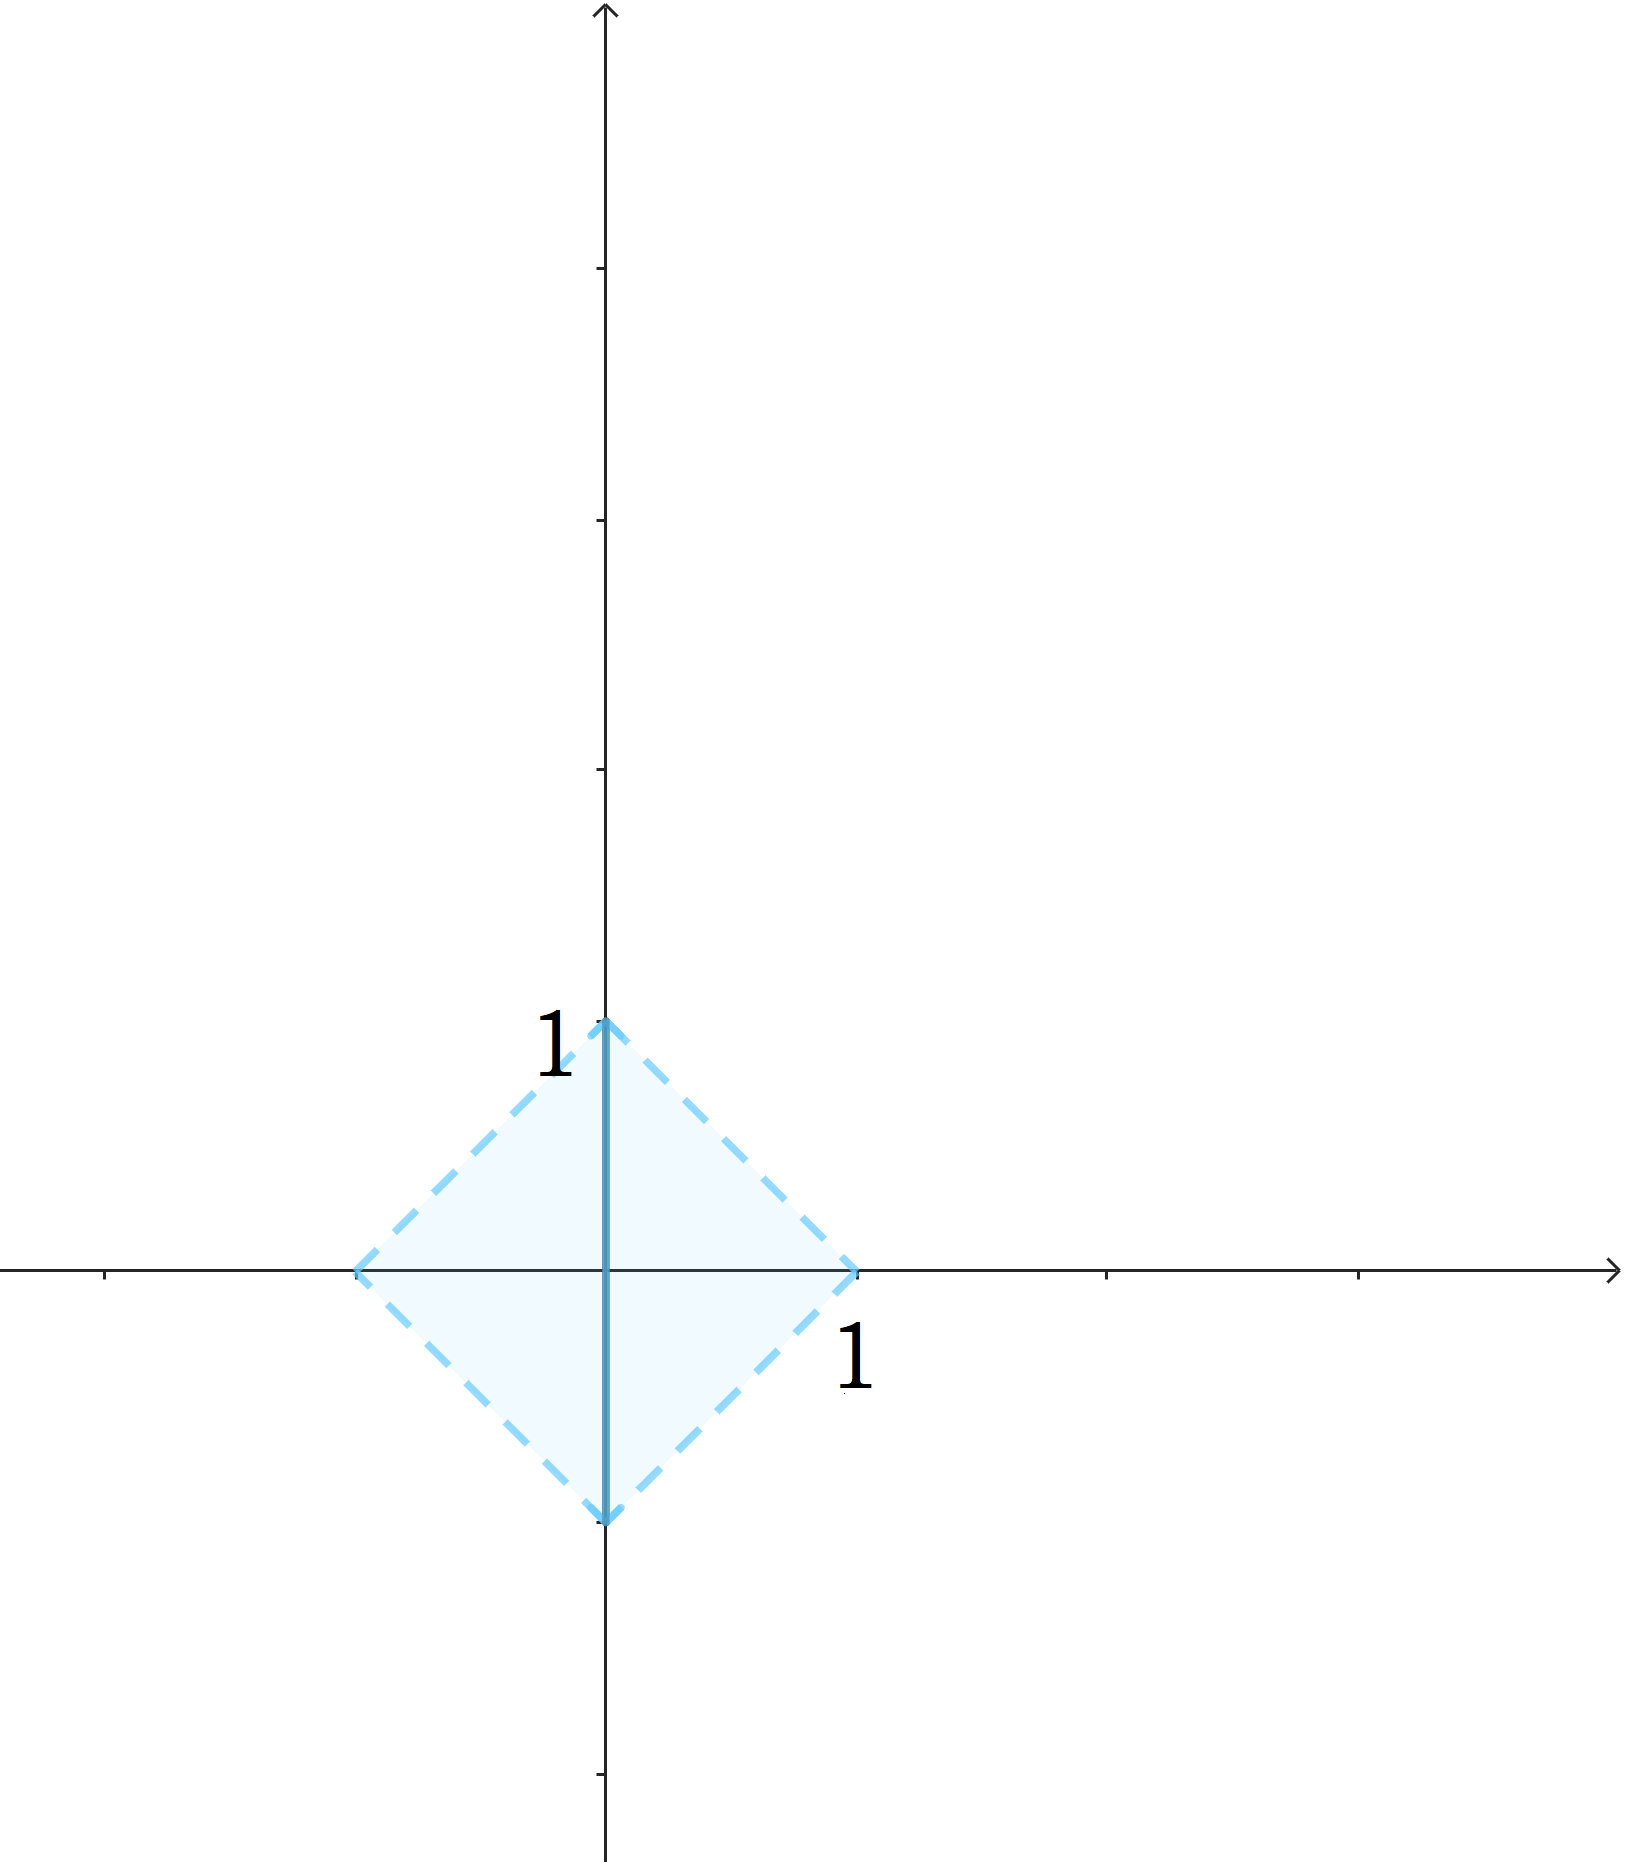
\includegraphics[scale=0.20] {graph7}
		\caption{\label{fig:7} Open ball $B((0,0), 1) $ in $\gamma$ metric }
	\end{figure}
	
	
	\begin{figure}
		\centering
		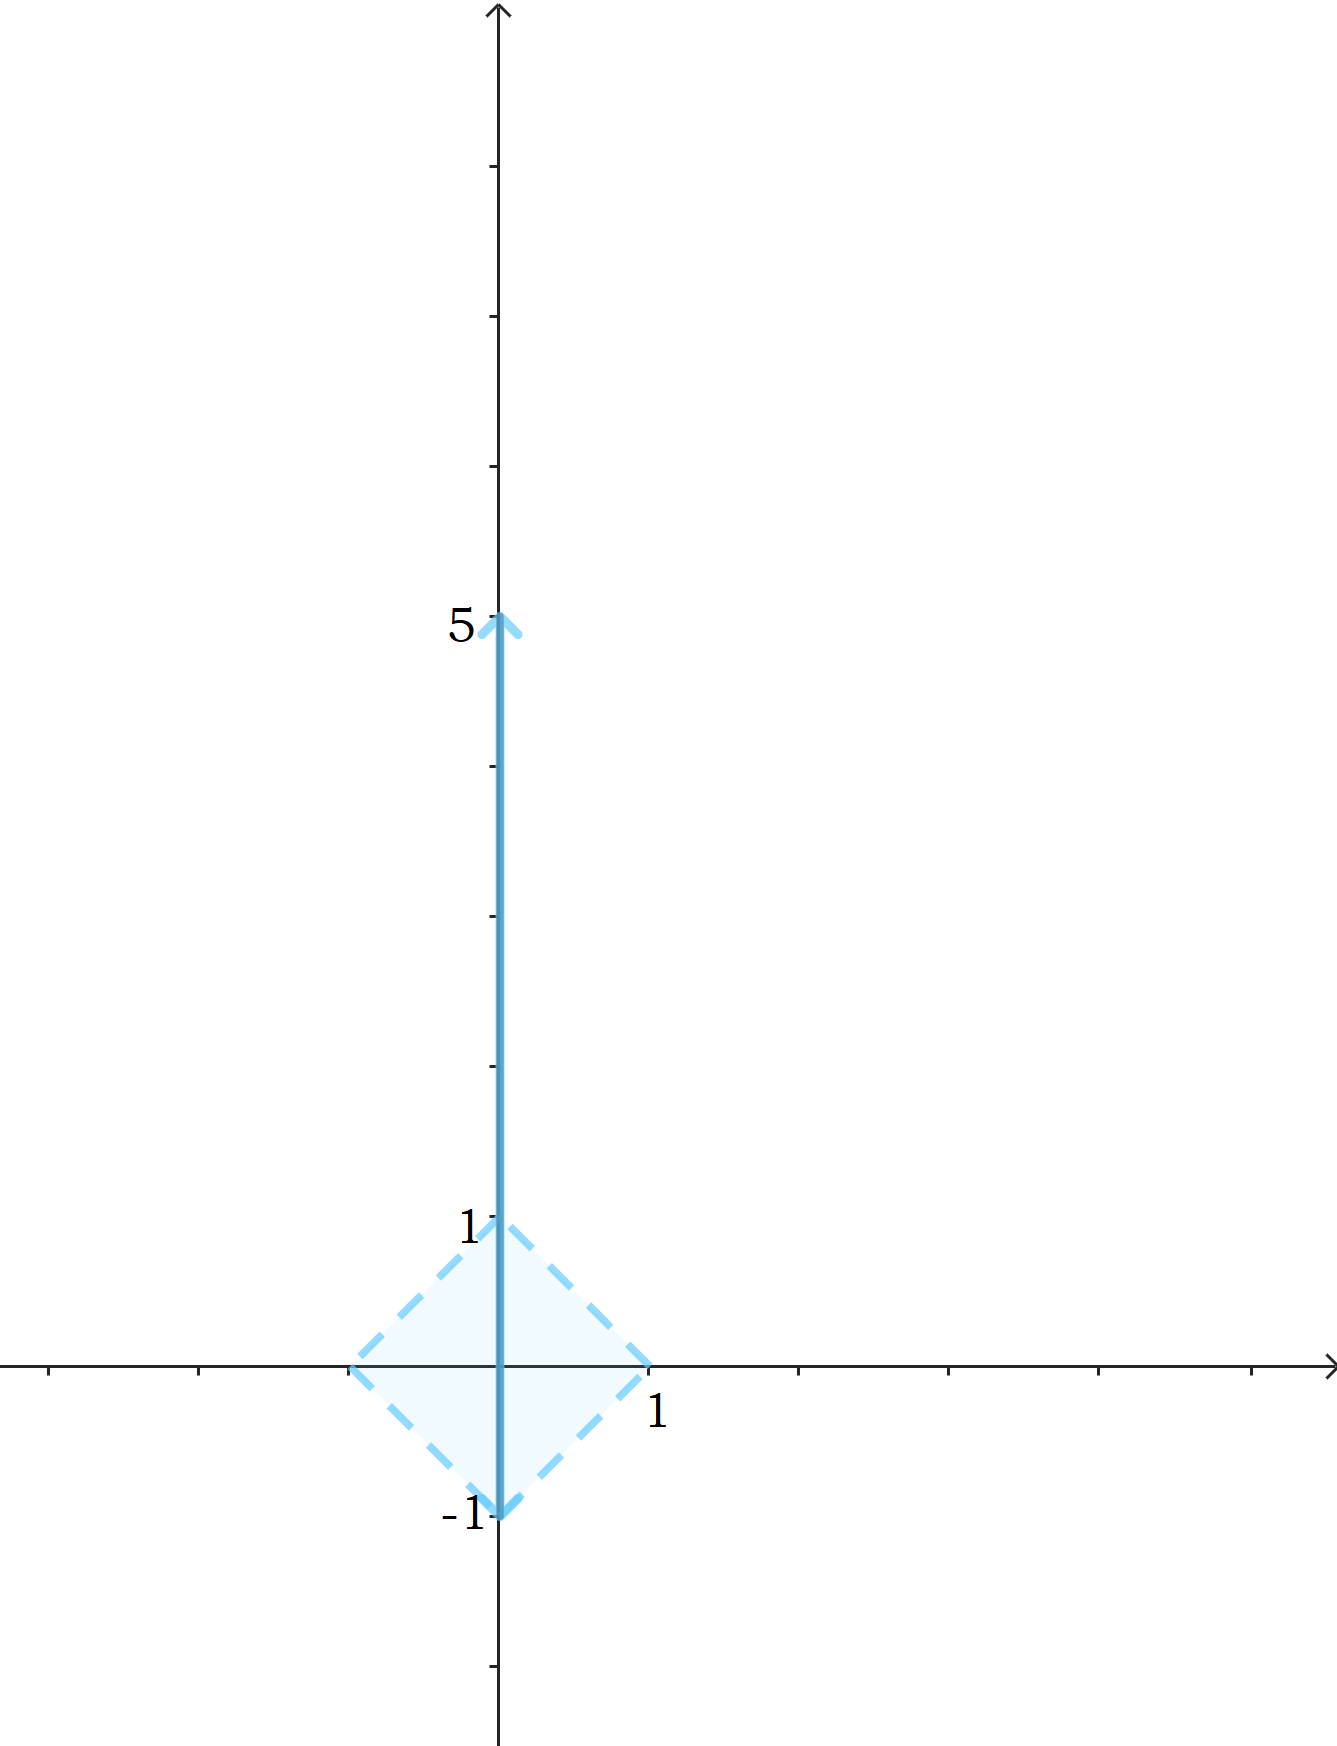
\includegraphics[scale=0.20] {graph8}
		\caption{\label{fig:8} Open ball $B((0,2), 3) $ in $\gamma$ metric }
	\end{figure}
	
	\begin{figure}
		\centering
		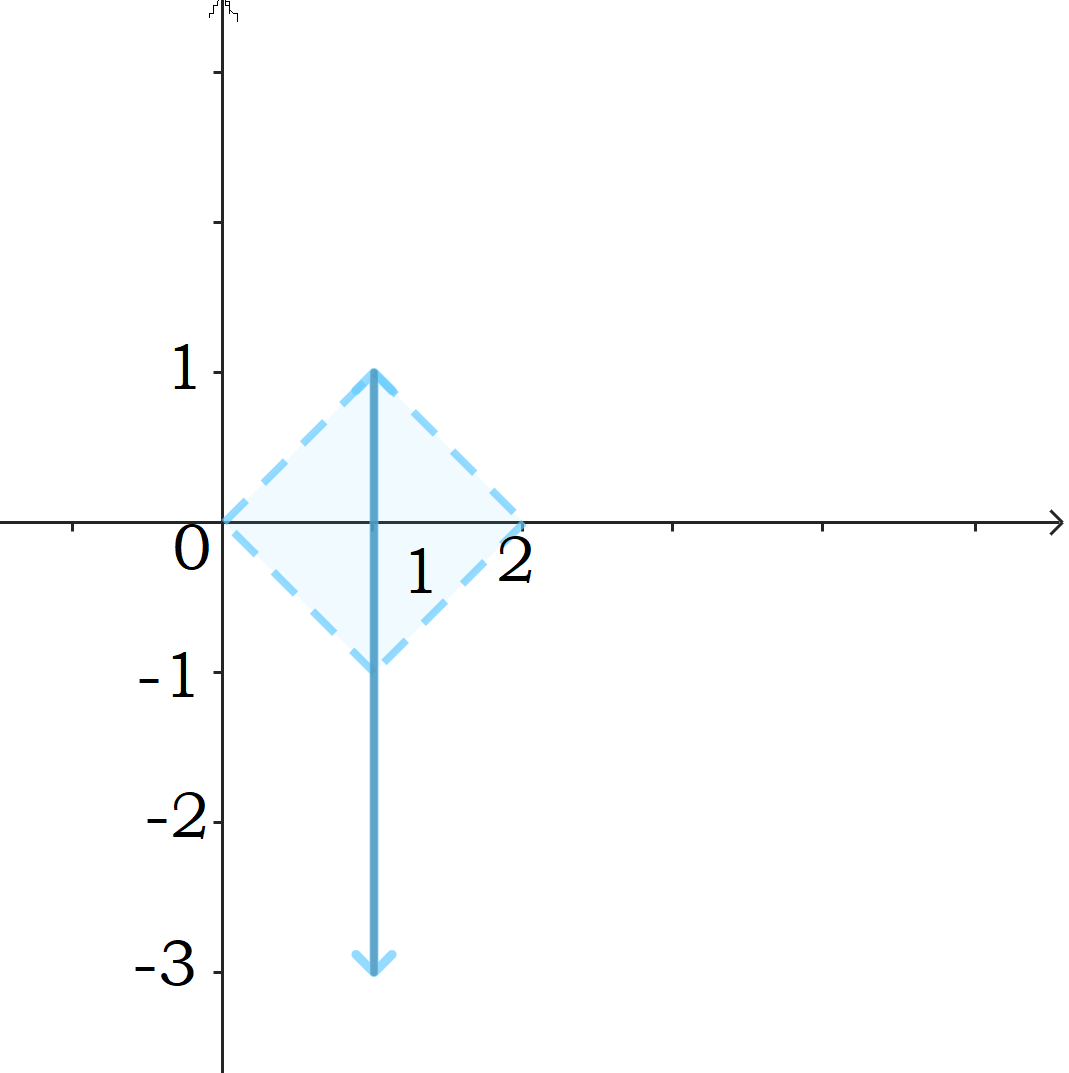
\includegraphics[scale=0.20] {graph9}
		\caption{\label{fig:9} Open ball $B((1,-1), 2) $ in $\gamma$ metric }
	\end{figure}
	\begin{align*}
		B((0,0), 1) &= \{(x_{1}, x_{2}) \in \mathbb{R}; \ \gamma((0,0),(x_{1}, x_{2}))<1\} \\
		&= \{(x_{1}, x_{2}) \in \mathbb{R}; \ x_{1} = 0 \land |x_{2}-0|<1\} \cup \{(x_{1}, x_{2}) \in \mathbb{R}; \ x_{1} \neq 0 \land |0| + |x_{1}-0| + |x{2}|<1\} \\
		&= \{(0, x_{2}) \in \mathbb{R}; \ \land \ |x_{2}|<1\} \cup \{(x_{1}, x_{2}) \in \mathbb{R}; \ x_{1} \neq 0 \land |x_{1}| + |x_{2}|<1\}
	\end{align*}

	\begin{align*}
	B((0,2), 3) &= \{(x_{1}, x_{2}) \in \mathbb{R}; \ \gamma((0,2),(x_{1}, x_{2}))<3\} \\
	&= \{(x_{1}, x_{2}) \in \mathbb{R}; \ x_{1} = 0 \land |x_{2}-2|<3\} \cup \{(x_{1}, x_{2}) \in \mathbb{R}; \ x_{1} \neq 0 \land |2| + |x_{1}-0| + |x{2}|<3\} \\
	&= \{(0, x_{2}) \in \mathbb{R}; \ \land \ |x_{2}-2|<3\} \cup \{(x_{1}, x_{2}) \in \mathbb{R}; \ x_{1} \neq 0 \land |x_{1}| + |x_{2}|<1\}
	\end{align*}

	\begin{align*}
		B((1,-1), 2) &= \{(x_{1}, x_{2}) \in \mathbb{R}; \ \gamma((1,-1),(x_{1}, x_{2}))<2\} \\
		&= \{(x_{1}, x_{2}) \in \mathbb{R}; \ x_{1} = 1 \land |x_{2}+1|<2\} \\
		&\cup \{(x_{1}, x_{2}) \in \mathbb{R}; \ x_{1} \neq 0 \land |-1| + |x_{1}-1| + |x{2}|<2\} \\
		&= \{(1, x_{2}) \in \mathbb{R}; \ \land \ |x_{2}+1|<2\} \cup \{(x_{1}, x_{2}) \in \mathbb{R}; \ x_{1} \neq 0 \land |x_{1}-1| + |x_{2}|<1\}
	\end{align*}
	

\subsection{Discrete metric} 
 \textbf{(a)}
    \begin{align*}
    	B(1,\frac{1}{2}) &= \{ x \in \mathbb{N}; d(1,x)<\frac{1}{2}\} \\
    	&= \{ x \in \mathbb{N}; x=1 \land 0<\frac{1}{2}\} \cup  \{ x \in \mathbb{N}; x \neq 1 \land d(1,x)<\frac{1}{2}\}  \\
    	&= \{1\} \cup \emptyset \\ 
    	&= \{1\}
    \end{align*}

 \begin{align*}
	B(2,1) &= \{ x \in \mathbb{N}; d(2,x)<1\} \\
	&= \{ x \in \mathbb{N}; x=2 \land 0<1\} \cup  \{ x \in \mathbb{N}; x \neq 2 \land d(2,x)<2\}  \\
	&= \{2\} \cup \emptyset \\ 
	&= \{2\}
\end{align*}

\begin{align*}
	\overline{B}(3,\frac{1}{2}) &= \{ x \in \mathbb{N}; d(3,x)\leq \frac{1}{2}\} \\
	&= \{ x \in \mathbb{N}; x=3 \land 0\leq \frac{1}{2}\} \cup  \{ x \in \mathbb{N}; x \neq 3 \land d(3,x)\leq \frac{1}{2}\}  \\
	&= \{3\} \cup \emptyset \\ 
	&= \{3\}
\end{align*}

\begin{align*}
	\overline{B}(4,1) &= \{ x \in \mathbb{N}; d(4,x)\leq 1\} \\
	&= \{ x \in \mathbb{N}; x=4 \land 0\leq1\} \cup  \{ x \in \mathbb{N}; x \neq 4 \land 1\leq 1\}  \\
	&= \{4\} \cup \mathbb{N} \setminus \{4\}\} \\ 
	&= \mathbb{N}
\end{align*}

In general, this discrete metric on space $X$ induces a metric space $(X,d)$ where the distance between any two pairwise distinct elements is $1$. Open and closed balls in this space contain one element or all of them:

\begin{equation*}
	B(x_{0}, r) =
	\begin{cases}
		\{x_{0}\} & 0 < r \leq 1\\
		 \mathbb{N} & r > 1\\
	\end{cases}       
\end{equation*}

\begin{equation*}
	\overline{B}(x_{0}, r) =
	\begin{cases}
		\{x_{0}\} & 0 < r < 1\\
		\mathbb{N} & r \geq 1\\
	\end{cases}       
\end{equation*}

\textbf{(b)} Because the distance between any two pairwise distinct elements is $1$, every triangle $abc$ with pairwise distinct elements $a$, $b$ and $c$ is equilateral (all three edges have the same lenght 1).

\subsection{Homeomorphic spaces} 
In this exercise I was working with spaces $X_{n} = ...$ and $Y_{n}=...$ \\

\noindent Spaces $X_{1}$, $Y_{1}$, $X_{2}$, $Y_{2}$ that I've drawn can be seen on Figures 10, 11 and 12. \\

\noindent I got the inspiration for the proof for a general $n$ from the solved problems book by asist. dr. Aleksandra Franc (2) on spletna učilnica where lies the proof for $n=2$. I generalized the idea for $n \in \mathbb{N}$. \\


\noindent In my proof I used the following theorem from the lectures: \\

\noindent \textbf{Theorem} Let $X$ and $Y$ be topological spaces. If we can find continuous maps $f : X \rightarrow Y$ and $g : Y \rightarrow X$ such that $f \circ g = id_{Y}$ and $g \circ f = id_{X}$, then X and Y are homeomorphic. \\

\noindent \textbf{Proof that $X_{n}$ and $Y_{n}$ are homeomorphic for any $n \in \mathbb{N}$:} \\






 
    
    
    
    
    
	
	\bibliographystyle{unsrt}
	\bibliography{references}
	
	
	
	% --------------------------------------------------------------
	%     You don't have to mess with anything below this line.
	% --------------------------------------------------------------
	
	
\end{document}    
